%%%%%%
% $Author: Kumari $
% $Date: 2023-01-22 $
%%%


\chapter{Getting started with ESP32}

	ESP32 is a microcontroller that has built-in WiFi and Bluetooth capabilities. It can be used to create a digital meter using various sensors and displays.\\
	
	To get started with using an ESP32 for a digital meter, you will first need to set up the development environment and install the necessary software, such as the Arduino IDE. Once this is done, you can upload a sketch (program) to the ESP32 that will control the sensors and display.\\
	
\begin{figure}  [H]
	\begin{center}
		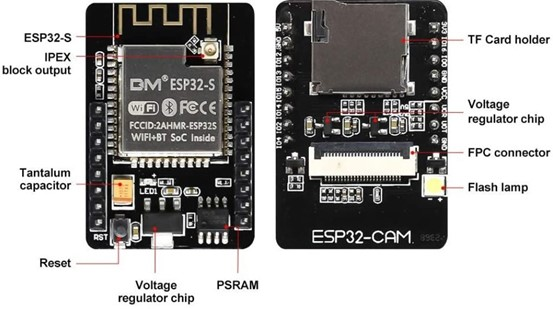
\includegraphics[width=12cm]{Chapters/ESP32components}
		\caption{Development board components in ESP32-CAM} 
		\label{fig:Components in ESP32 Cam}
		\footnotesize \textbf{Reference:} \autocite{Lab:2021}
	\end{center}
\end{figure}

Following figure shows the output and power pins. There are three GND pins and two pins for power, it could be 3.3V or 5V. To upload the code, two serial pins GPIO1 and GPIO3 are used. GPIO0 is used to check the flash mode. To be able to upload code, GPIO0 should be connected to GND \autocite{randomnerdtutorials}.

\begin{figure}  [H]
	\begin{center}
		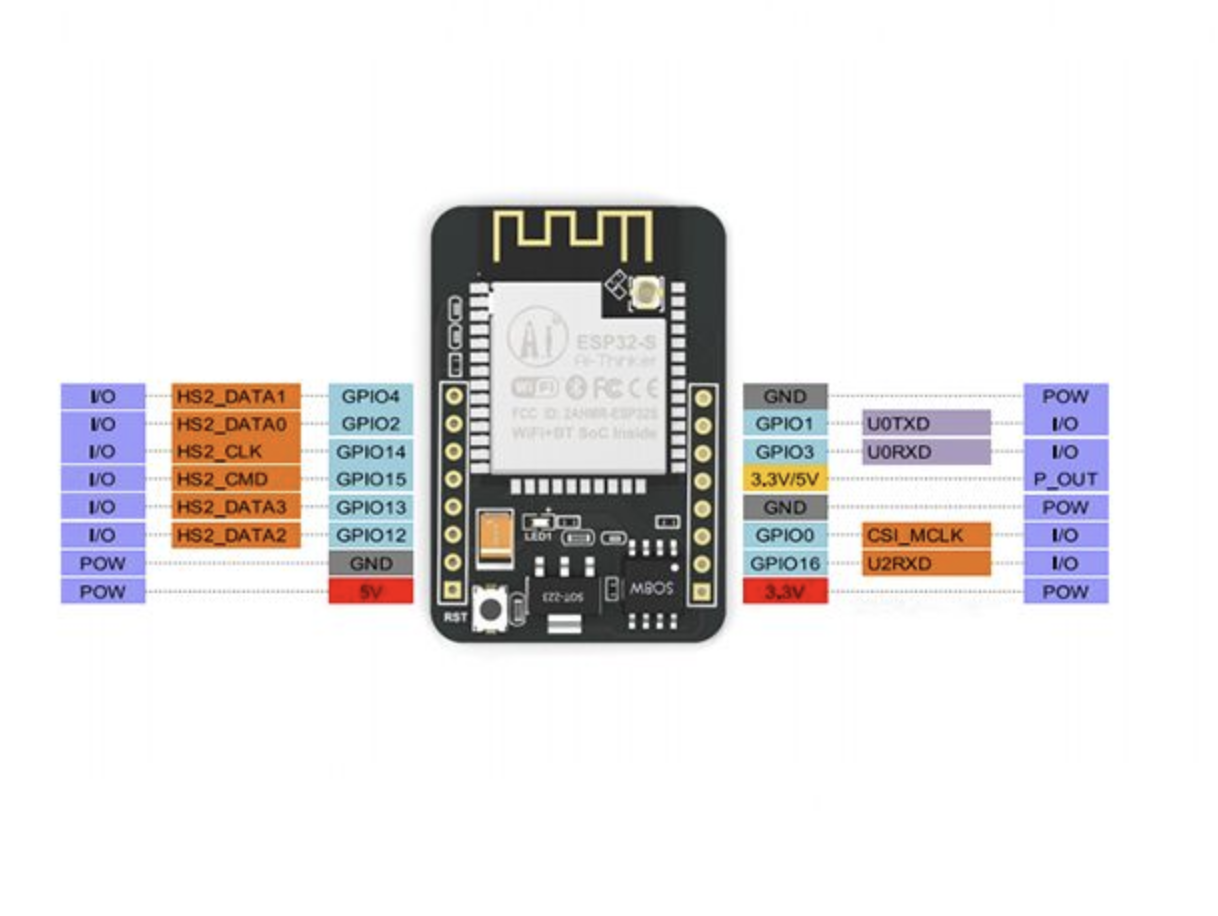
\includegraphics[width=12cm]{Chapters/ESP32CAMpinout}
		\caption{ESP32 CAM PINOUT} 
		\label{fig:Components in ESP32 Cam}
		\footnotesize \textbf{Reference:} \autocite{randomnerdtutorials}
	\end{center}
\end{figure}

	
\section{Functions}
	The main function of a digital meter created using an ESP32 would be to read sensor data, process that data, and display it on a screen. The sketch for the digital meter would likely include code to handle communication with the sensors, code to process the data, and code to display it on the screen.\\
	
	The GUI or UI of the digital meter would depend on the specific implementation. It could include a simple numerical display, or it could include more advanced features such as graphs or charts.\\
	
	In this project, we prefer a numerical display.\\
	
\section{Specifications}

\begin{itemize}
	\item Processing power of up to 240 MHz dual core
	\item Wi-Fi - 802.11b/g/n/e/i
	\item Bluetooth 4.2 BR/EDR and BLE standards
	\item Up to 520 KB SRAM
	\item Up to 4MB flash memory
	\item 40-pin GPIO header
\end{itemize}

More detailed specifications and hardware decsriptions are already mentioned in ESP32 section under DomainKnowledge chapter of the team report.

\section{Independence of internals}
The independence of the internals would depend on the specific implementation of the digital meter using the ESP32. It could be designed to operate independently or to communicate with other devices.\\

The internal peripherals, such as the Analog-to-Digital Converter or the Inter-Integrated Circuit controller operate independently of the main processor. The digitization of analog meter readings without the need for additional external components is possible.